\section{The Zeeman effect}

\begin{frame}{About concepts}
\uncover<1->{
    \begin{block}{Original concepts}
        A atomic spectral lines split in an external magnetic field:
        \begin{equation*}
            \begin{cases}
                    3: \text{The normal Zeeman effect}.\\
                    \text{the other}: \text{The anomalous Zeeman effect}.
            \end{cases}
        \end{equation*}
    \end{block}}
\uncover<2->{
    Modern:\\
    In a strong field: Paschen-Back effect.\\
    In a weak field:
    \begin{equation*}
        \begin{cases}
                3: \text{The normal Zeeman effect}.\\
                \text{the other}: \text{The anomalous Zeeman effect}.
            \end{cases}
    \end{equation*}
    }
\end{frame}

\subsection{The Paschen-Back effect}

\begin{frame}{The Paschen-Back effect}
\uncover<1->{
    For LS-coupling scheme, the atom's magnetic moment:
    \begin{equation*}
        \boldsymbol{\mu}=-\mu_{\mathrm{B}}\boldsymbol{L}-g_{s}\mu_{\mathrm{B}}\boldsymbol{S}.
    \end{equation*}}
\uncover<2->{
    The interaction of the atom with an external magnetic field is described by
    \begin{equation*}
        H_{{\mathrm{ZE}}}=-\boldsymbol{\mu}\cdot\boldsymbol{B}.
    \end{equation*}}
\uncover<3->{
    In a strong field: consider total magnetic moment along the z-direction
    \begin{equation*}
        \mu_z=\mu_{sz}+\mu_{lz}=-2\mu_\mathrm{B}m_s-\mu_\mathrm{B}m_l=-(2m_s+m_l)\mu_\mathrm{B}.
    \end{equation*}}
\uncover<4->{
    Energy: 
    \begin{equation*}
        E_{\mathrm{ZE}}=-\mu_\mathrm{z}B=(2m_s+m_l)\mu_\mathrm{B}.
    \end{equation*}}
\uncover<5->{
    \begin{block}{Selection rules}
        \begin{equation*}
            \begin{cases}
                \Delta m_s=0\\
                \Delta m_l=0,\pm1
            \end{cases}
        \end{equation*}
    \end{block}}
\end{frame}

\begin{frame}{Example}
    \begin{figure}
        \centering
        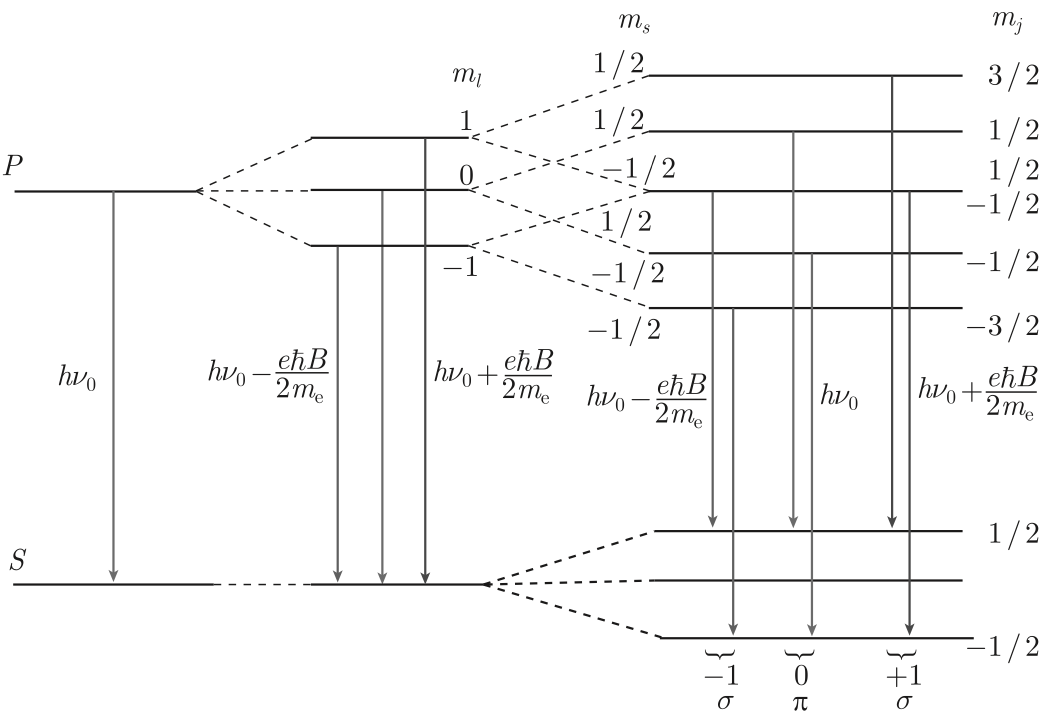
\includegraphics[scale=0.4]{fig/fig 5.13.png}
        \caption{$m_l=1, m_s=-\dfrac{1}{2},m_j=\dfrac{1}{2}$\&$m_l=-1,m_s=\dfrac{1}{2},m_j=-\dfrac{1}{2}$ are degenerate}
    \end{figure}
\end{frame}

\begin{frame}{The Zeeman effect}
\uncover<1->{
    In weak magnetic field, Hamiltonian: 
    \begin{equation*}
        H_{{\mathrm{ZE}}}=-\frac{\langle\boldsymbol{\mu}\cdot\boldsymbol{J}\rangle}{J\left(J+1\right)}\boldsymbol{J}\cdot\boldsymbol{B}=\frac{\langle\boldsymbol{L}\cdot\boldsymbol{J}\rangle+g_{s}\left\langle\boldsymbol{S}\cdot\boldsymbol{J}\right\rangle}{J\left(J+1\right)}\mu_{{\mathrm{B}}}BJ_{z}.
    \end{equation*}}
\uncover<2->{
    Energy: 
    \begin{equation*}
        E_{\mathrm{ZE}}=g_{J}\mu_{\mathrm{B}}BM_{J}.
    \end{equation*}}
\uncover<3->{
    Lande $g$-factor: 
    \begin{equation*}
        g_J=\frac{\langle\boldsymbol{L}\cdot\boldsymbol{J}\rangle+g_{s}\left\langle\boldsymbol{S}\cdot\boldsymbol{J}\right\rangle}{J\left(J+1\right)}.
    \end{equation*}
    }
\uncover<4->{
    Assuming that $g_s\simeq2$:
    \begin{equation*}
        g_J=\frac32+\frac{S\left(S+1\right)-L\left(L+1\right)}{2J\left(J+1\right)}.
    \end{equation*}
    }
\end{frame}

\begin{frame}{The Zeeman effect}
\uncover<1->{
    \begin{block}{No magnetic field}
        Consider $2\to1$:
        \begin{equation*}
            h\nu=E_2-E_1.
        \end{equation*}
    \end{block}}
\uncover<2->{
    External magnetic field $\boldsymbol{B}$:
    \begin{equation*}
        E_2'=E_2+g_2M_{J2}\mu_\text{B}B,\quad E_1'=E_1+g_1M_{J1}\mu_\text{B}B.
    \end{equation*}}
\uncover<3->{
    Spectral line splitting:
    \begin{equation*}
        E_2^{\prime}-E_1^{\prime}=h\nu+\left(g_2M_{J2}-g_1M_{J1}\right)\mu_\mathrm{B}B.
    \end{equation*}}
\uncover<4->{
    \begin{block}{Selection rules}
        \begin{equation*}
        \Delta M_J=0,\pm1.
    \end{equation*}
    \end{block}}
\end{frame}

\subsection{The normal Zeeman effect}

\begin{frame}{The normal Zeeman effect}
    \begin{figure}
        \centering
        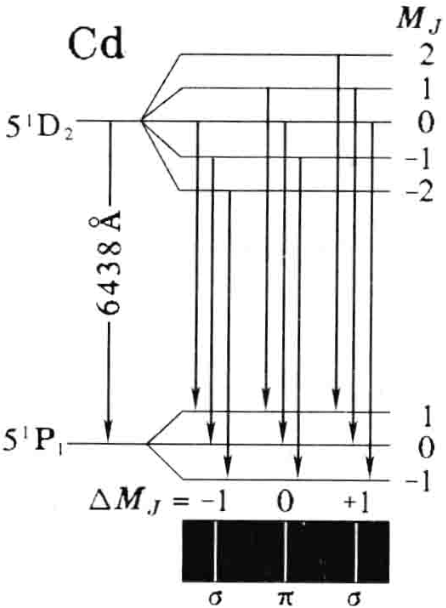
\includegraphics[scale=0.6]{fig/fig 5.14.png}
        \caption{Cd $5^1$D$_2\to5^1$P$_1:\,S_1=S_2=0\Rightarrow g_1=g_2=1$}
    \end{figure}
\end{frame}

\subsection{The anomalous Zeeman effect}

\begin{frame}{The anomalous Zeeman effect}
    \begin{figure}
        \centering
        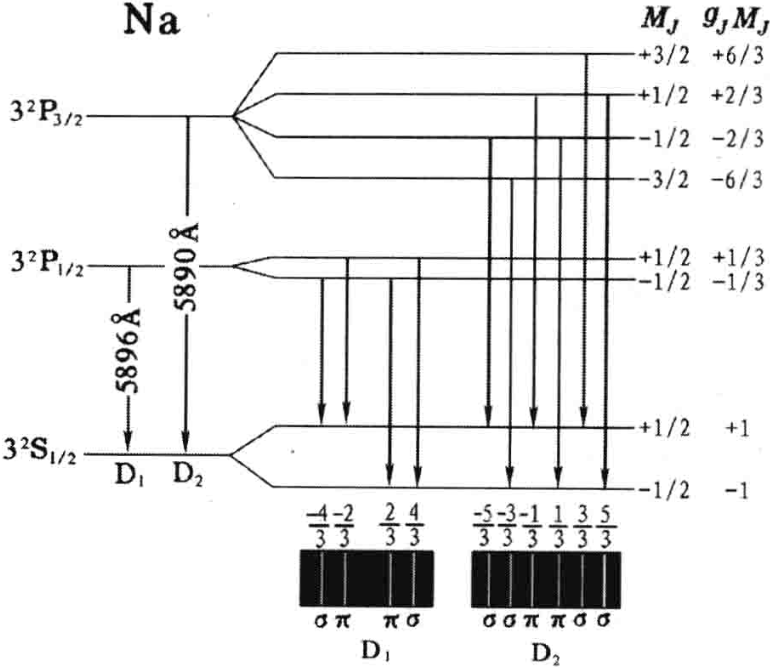
\includegraphics[scale=0.5]{fig/fig 5.15.png}
        \caption{Na $3^2$P$_{3/2}\to3^2$S$_{1/2}$/ $3^2$P$_{1/2}\to3^2$S$_{1/2}$}
    \end{figure}
\end{frame}